\documentclass[12pt,a4paper]{article}

% ─── Packages ─────────────────────────────────────────────────────────────
\usepackage[utf8]{inputenc}
\usepackage[T1]{fontenc}
\usepackage{amsmath,amssymb,amsthm}
\usepackage{mathtools}
\usepackage[margin=1in]{geometry}
\usepackage{hyperref}
\usepackage{xcolor}
\usepackage{booktabs}
\usepackage{enumitem}
\usepackage{fancyhdr}
\usepackage{graphicx}
\usepackage{float}
\usepackage{tikz}
\usepackage{tcolorbox}
\usetikzlibrary{arrows.meta,positioning,shapes.geometric,decorations.pathreplacing,calc}

% Path to presentation figures
\graphicspath{{results/images/presentation/}}

% ─── Custom commands ──────────────────────────────────────────────────────
\newcommand{\abs}[1]{\left|#1\right|}
\newcommand{\Real}{\operatorname{Re}}
\newcommand{\Imag}{\operatorname{Im}}
\newcommand{\FFT}{\operatorname{FFT}}
\newcommand{\IFFT}{\operatorname{IFFT}}
\DeclareMathOperator{\sech}{sech}
\newcommand{\pdv}[2]{\frac{\partial #1}{\partial #2}}
\newcommand{\dv}[2]{\frac{d #1}{d #2}}

% ─── Colored boxes ────────────────────────────────────────────────────────
\newtcolorbox{intuition}{colback=blue!5,colframe=blue!40!black,title=\textbf{Intuition}}
\newtcolorbox{keyeq}{colback=green!5,colframe=green!50!black,title=\textbf{Key Equation}}
\newtcolorbox{mlbox}{colback=orange!5,colframe=orange!50!black,title=\textbf{ML Connection}}
\newtcolorbox{warning}{colback=red!5,colframe=red!50!black,title=\textbf{Watch Out}}

% ─── Header/Footer ────────────────────────────────────────────────────────
\pagestyle{fancy}
\fancyhf{}
\fancyhead[L]{\small Companion Explainer --- Rivera Lab}
\fancyhead[R]{\small\thepage}
\fancyfoot[C]{\small Understanding the Math Behind Raman Suppression --- \today}

% ═════════════════════════════════════════════════════════════════════════
\title{\textbf{The Companion Explainer}\\[6pt]
Understanding the Math Behind\\
Raman Suppression via Spectral Phase Optimization\\[12pt]
\large A First-Principles Walkthrough for Undergrads\\[6pt]
\normalsize Rivera Lab, Cornell University}
\author{Companion to the Verification Document\\
\small Prepared for Ignacio Rivera}
\date{April 2026}

\begin{document}
\maketitle
\thispagestyle{empty}

\begin{abstract}
This document explains every piece of math in the Raman suppression optimization project, starting from Maxwell's equations and building up to the adjoint method and the log-scale cost function. It's written for an undergrad physics major who knows Fourier transforms, wave equations, and complex numbers --- and wants to understand \emph{why} each equation is the way it is, not just \emph{what} it says.

\medskip\noindent\textbf{How to read this:} Parts 1--3 give you the physics and the optimization setup. Part 4 is the key insight (the adjoint method). Parts 5--8 cover the tricks that make it work in practice. Parts 9--10 show how we verify correctness. Parts 11--13 go deeper: the ML connection, the GNLSE from Maxwell's equations, and the adjoint from the Lagrangian.

\medskip\noindent\textbf{Prerequisite:} Fourier transforms, basic complex numbers, the wave equation. That's it.
\end{abstract}

\tableofcontents
\newpage

% ═════════════════════════════════════════════════════════════════════════
\section{The Big Picture (No Math Yet)}

Imagine a laser pulse --- a burst of light lasting 185 femtoseconds (185$\times 10^{-15}$~s) --- traveling through an optical fiber. The fiber is glass (SiO$_2$), and the glass has atoms that vibrate. When the intense pulse hits these atoms, some of the light's energy excites the vibrations and gets re-emitted at a lower frequency. This is \textbf{Raman scattering}: light loses energy and shifts to redder colors.

Three things happen simultaneously as the pulse propagates:
\begin{enumerate}
    \item \textbf{Dispersion:} Different colors travel at different speeds. The pulse spreads out.
    \item \textbf{Kerr effect:} The light is so intense it changes the glass's refractive index. The pulse modifies its own phase.
    \item \textbf{Raman scattering:} The glass steals energy and red-shifts it.
\end{enumerate}

\textbf{Our approach:} Before the pulse enters the fiber, we reshape its \emph{spectral phase} using a pulse shaper --- a device that delays different colors by different amounts. By choosing the right delay pattern, we make the pulse propagate through the fiber in a way that minimizes Raman scattering.

\begin{intuition}
We can only control the \emph{timing} of different colors, not which colors are present. It's like adjusting when each runner starts in a relay race, but not which runners participate. The timing determines the temporal shape of the pulse, which determines how it interacts with the glass.
\end{intuition}


% ─── Pipeline diagram ─────────────────────────────────────────────────────
\begin{figure}[H]
\centering
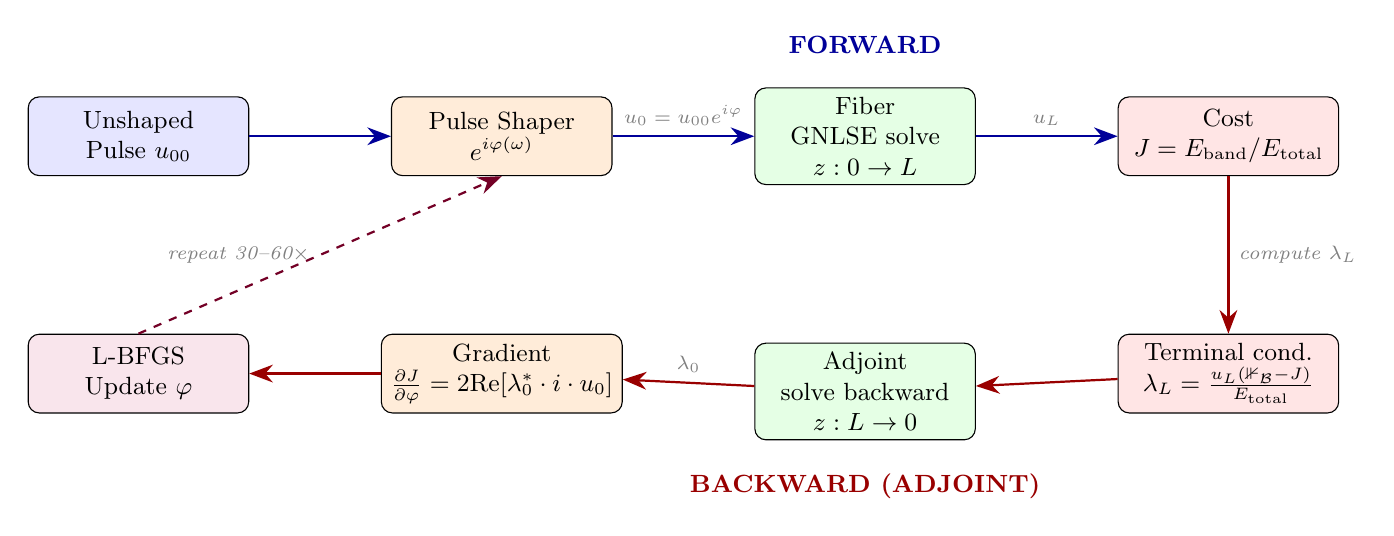
\begin{tikzpicture}[
    node distance=1.2cm and 1.8cm,
    box/.style={rectangle, draw, rounded corners, minimum width=2.8cm, minimum height=1cm, align=center, font=\small},
    arrow/.style={-{Stealth[length=3mm]}, thick},
    label/.style={font=\scriptsize\itshape, text=gray}
]
% Forward path (top)
\node[box, fill=blue!10] (pulse) {Unshaped\\Pulse $u_{00}$};
\node[box, fill=orange!15, right=of pulse] (shaper) {Pulse Shaper\\$e^{i\varphi(\omega)}$};
\node[box, fill=green!10, right=of shaper] (fiber) {Fiber\\GNLSE solve\\$z: 0 \to L$};
\node[box, fill=red!10, right=of fiber] (cost) {Cost\\$J = E_{\text{band}}/E_{\text{total}}$};

\draw[arrow, blue!60!black] (pulse) -- (shaper);
\draw[arrow, blue!60!black] (shaper) -- node[above, label] {$u_0 = u_{00}e^{i\varphi}$} (fiber);
\draw[arrow, blue!60!black] (fiber) -- node[above, label] {$u_L$} (cost);

% Backward path (bottom)
\node[box, fill=red!10, below=2cm of cost] (terminal) {Terminal cond.\\$\lambda_L = \frac{u_L(\mathbb{1}_\mathcal{B} - J)}{E_{\text{total}}}$};
\node[box, fill=green!10, below=2cm of fiber] (adjoint) {Adjoint\\solve backward\\$z: L \to 0$};
\node[box, fill=orange!15, below=2cm of shaper] (gradient) {Gradient\\$\frac{\partial J}{\partial\varphi} = 2\text{Re}[\lambda_0^* \cdot i \cdot u_0]$};
\node[box, fill=purple!10, below=2cm of pulse] (update) {L-BFGS\\Update $\varphi$};

\draw[arrow, red!60!black] (cost) -- node[right, label] {compute $\lambda_L$} (terminal);
\draw[arrow, red!60!black] (terminal) -- (adjoint);
\draw[arrow, red!60!black] (adjoint) -- node[above, label] {$\lambda_0$} (gradient);
\draw[arrow, red!60!black] (gradient) -- (update);

% Loop back
\draw[arrow, purple!60!black, thick, dashed] (update.north) -- (shaper.south) node[midway, left, label] {repeat 30--60$\times$};

% Labels
\node[above=0.3cm of fiber, font=\small\bfseries, blue!60!black] {FORWARD};
\node[below=0.3cm of adjoint, font=\small\bfseries, red!60!black] {BACKWARD (ADJOINT)};
\end{tikzpicture}
\caption{The optimization pipeline. Blue arrows: forward propagation computes the cost. Red arrows: adjoint propagation computes the gradient. Purple dashed: L-BFGS updates the phase and repeats. One full cycle takes ${\sim}2$~seconds.}
\label{fig:pipeline}
\end{figure}


% ═════════════════════════════════════════════════════════════════════════
\section{The Wave Equation (The GNLSE)}

\subsection{From Maxwell's Equations to One Equation}

You've seen the wave equation:
\begin{equation}
\frac{\partial^2 E}{\partial z^2} = \frac{1}{c^2}\frac{\partial^2 E}{\partial t^2}
\end{equation}

For light in a fiber, we need three modifications: frequency-dependent speed (dispersion), intensity-dependent refractive index (Kerr), and energy transfer between frequencies (Raman). The result is the \textbf{Generalized Nonlinear Schr\"odinger Equation (GNLSE)}:

\begin{keyeq}
\begin{equation}
\pdv{u}{z} = \underbrace{iD(\omega)\cdot u}_{\text{dispersion}} + \underbrace{i\gamma(1-f_R)|u|^2 u}_{\text{Kerr}} + \underbrace{i\gamma f_R\,(h_R * |u|^2)\,u}_{\text{Raman}}
\label{eq:gnlse}
\end{equation}
\end{keyeq}

\subsection{What Each Term Means}

\textbf{The field $u(z,t)$} is the complex envelope of the electric field. $|u|^2$ gives instantaneous power in Watts. It depends on position $z$ along the fiber and time $t$.

\textbf{Dispersion $iD(\omega)u$:} Each color $\omega$ picks up phase $D(\omega)\cdot z$ per meter:
\begin{equation}
D(\omega) = \frac{\beta_2}{2}\omega^2 + \frac{\beta_3}{6}\omega^3 + \cdots
\end{equation}
\begin{itemize}
    \item $\beta_2$ = group velocity dispersion. Negative $\Rightarrow$ anomalous dispersion (longer wavelengths faster).
    \item $\beta_3$ = third-order dispersion. Usually a small correction.
\end{itemize}
Think of $D(\omega)$ as a recipe: ``delay blue by this much, delay red by that much, per meter of fiber.''

\textbf{Kerr effect $i\gamma|u|^2 u$:} The refractive index changes as $n = n_0 + n_2|E|^2$. The pulse phase shifts proportionally to its own intensity. The constant $\gamma$ (gamma) measures the fiber's nonlinear strength:
\begin{center}
\begin{tabular}{ll}
SMF-28: & $\gamma = 0.0011$ W$^{-1}$m$^{-1}$ (weakly nonlinear) \\
HNLF:   & $\gamma = 0.010$ W$^{-1}$m$^{-1}$ (10$\times$ stronger)
\end{tabular}
\end{center}

\textbf{Raman effect $i\gamma f_R(h_R * |u|^2)u$:} The glass responds with a delay --- atoms take ${\sim}30$~fs to ring up. The response function $h_R(t)$ is a damped oscillation:
\begin{equation}
h_R(t) = \frac{\tau_1^2 + \tau_2^2}{\tau_1\tau_2^2}\,e^{-t/\tau_2}\sin(t/\tau_1)\cdot\Theta(t)
\end{equation}
where $\tau_1 = 12.2$~fs (oscillation), $\tau_2 = 32$~fs (decay), and $\Theta(t)$ is the Heaviside function (causality: glass responds \emph{after} being hit). The $*$ means convolution --- the Raman response depends on the intensity history over the previous ${\sim}100$~fs. The fraction $f_R = 0.18$ means 18\% Raman (delayed), 82\% Kerr (instantaneous).

\subsection{The Interaction Picture}

\begin{intuition}
The dispersion term causes rapid oscillations that waste the ODE solver's time. It's like simulating a vibrating guitar string by tracking every oscillation when you only care about the slowly-changing envelope. The fix: go to a ``rotating frame'' (the interaction picture) where dispersion vanishes.
\end{intuition}

Define a new variable that ``rotates with'' the dispersion:
\begin{equation}
\tilde{u}_\omega(z) = e^{-iD(\omega)z}\cdot u_\omega(z)
\end{equation}

This is exactly like a rotating reference frame in classical mechanics. In this frame, only the nonlinear terms remain:
\begin{equation}
\dv{\tilde{u}_\omega}{z} = i\cdot e^{-iDz}\cdot[\text{nonlinear terms in the lab frame}]\cdot e^{+iDz}
\end{equation}

The ODE solver can now take large steps. To recover the physical field: $u_\omega = e^{+iDz}\tilde{u}_\omega$.


% ─── Interaction picture diagram ─────────────────────────────────────────
\begin{figure}[H]
\centering
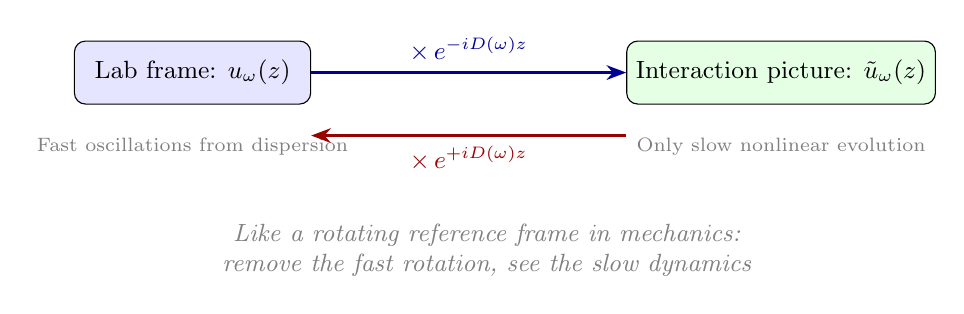
\begin{tikzpicture}[
    node distance=1cm,
    box/.style={rectangle, draw, rounded corners, minimum width=3cm, minimum height=0.8cm, align=center, font=\small},
    arrow/.style={-{Stealth[length=2.5mm]}, thick}
]
% Lab frame
\node[box, fill=blue!10] (lab) {Lab frame: $u_\omega(z)$};
\node[below=0.3cm of lab, font=\scriptsize, text=gray] {Fast oscillations from dispersion};

% Transform
\node[box, fill=green!10, right=4cm of lab] (ip) {Interaction picture: $\tilde{u}_\omega(z)$};
\node[below=0.3cm of ip, font=\scriptsize, text=gray] {Only slow nonlinear evolution};

% Arrows
\draw[arrow, blue!60!black] (lab) -- node[above, font=\small] {$\times\, e^{-iD(\omega)z}$} (ip);
\draw[arrow, red!60!black] ([yshift=-0.8cm]ip.west) -- node[below, font=\small] {$\times\, e^{+iD(\omega)z}$} ([yshift=-0.8cm]lab.east);

% Analogy
\node[below=1.8cm of $(lab)!0.5!(ip)$, font=\small\itshape, text=gray, align=center] {Like a rotating reference frame in mechanics:\\remove the fast rotation, see the slow dynamics};
\end{tikzpicture}
\caption{The interaction picture removes fast dispersive oscillations, letting the ODE solver take larger steps. Transform to lab frame when you need the physical field.}
\label{fig:interaction_picture}
\end{figure}


% ═════════════════════════════════════════════════════════════════════════
\section{The Optimization Problem}

\subsection{What We Control}

A pulse shaper applies a spectral phase $\varphi(\omega)$:
\begin{equation}
u_0(\omega) = u_{00}(\omega)\cdot e^{i\varphi(\omega)}
\label{eq:phase_mask}
\end{equation}
where $u_{00}$ is the original pulse. This changes the temporal shape without changing the power spectrum ($|u_0|^2 = |u_{00}|^2$).

\subsection{What We Minimize}

After propagation, measure the fractional energy in the Raman band:
\begin{keyeq}
\begin{equation}
J[\varphi] = \frac{\displaystyle\sum_{\omega\in\mathcal{B}}|u_L(\omega)|^2}{\displaystyle\sum_\omega |u_L(\omega)|^2} = \frac{E_{\text{band}}}{E_{\text{total}}}
\label{eq:cost}
\end{equation}
where $\mathcal{B}$ = frequencies shifted $> 5$~THz red of pump. $J = 0$ is perfect suppression.
\end{keyeq}

In decibels: $J_{\text{dB}} = 10\log_{10}(J)$. Our best: $-78$~dB $= 1.6\times10^{-8}$.

\subsection{The Landscape}

$J$ depends on $\varphi(\omega)$ --- a vector with $N_t = 8192$ components. We need to find the $\varphi$ that minimizes $J$ in this 8192-dimensional space. For that, we need the \textbf{gradient}: a vector pointing in the direction of steepest descent.


% ═════════════════════════════════════════════════════════════════════════
\section{How Optimization Works: From Gradient Descent to L-BFGS}

This section builds up the optimization algorithm from first principles. If you've taken multivariable calculus, you already know the core ideas.

\subsection{Gradient Descent: The Simplest Method}

You're standing on a hilly landscape in fog. You can't see far, but you can feel the slope under your feet. The obvious strategy: take a step in the downhill direction.

Mathematically, if $\varphi$ is your current position (the spectral phase vector) and $\nabla J$ is the gradient (the ``slope'' in each direction), then:
\begin{equation}
\varphi_{\text{new}} = \varphi_{\text{old}} - \alpha\,\nabla J
\label{eq:gd}
\end{equation}
where $\alpha > 0$ is the \textbf{step size} (or ``learning rate'' in ML). This is gradient descent.

\begin{warning}
\textbf{The step size problem.} If $\alpha$ is too large, you overshoot the minimum and bounce around. If too small, convergence takes forever. Worse: different directions may need different step sizes. Imagine a long, narrow valley --- you need large steps along the valley floor but tiny steps perpendicular to it. Gradient descent with a single $\alpha$ zig-zags, wasting most of its effort.
\end{warning}

% ─── Gradient descent zig-zag diagram ─────────────────────────────────────
\begin{figure}[H]
\centering
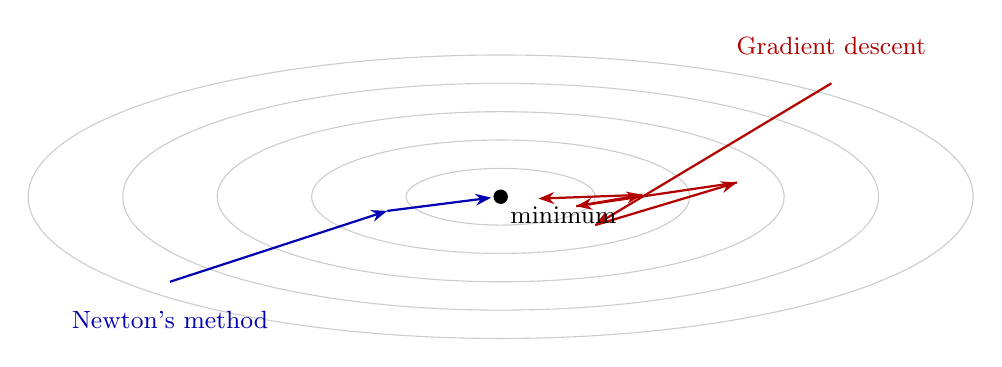
\begin{tikzpicture}[scale=1.2]
    % Elliptical contours
    \foreach \r in {0.5, 1.0, 1.5, 2.0, 2.5} {
        \draw[gray!40] (0,0) ellipse ({\r*2} and {\r*0.6});
    }
    % Gradient descent path (zig-zag)
    \draw[thick, red!70!black, -{Stealth[length=2mm]}] (3.5, 1.2) -- (1.0, -0.3);
    \draw[thick, red!70!black, -{Stealth[length=2mm]}] (1.0, -0.3) -- (2.5, 0.15);
    \draw[thick, red!70!black, -{Stealth[length=2mm]}] (2.5, 0.15) -- (0.8, -0.1);
    \draw[thick, red!70!black, -{Stealth[length=2mm]}] (0.8, -0.1) -- (1.5, 0.02);
    \draw[thick, red!70!black, -{Stealth[length=2mm]}] (1.5, 0.02) -- (0.4, -0.02);
    \node[red!70!black, font=\small] at (3.5, 1.6) {Gradient descent};

    % Newton's method path (direct)
    \draw[thick, blue!70!black, -{Stealth[length=2mm]}] (-3.5, -0.9) -- (-1.2, -0.15);
    \draw[thick, blue!70!black, -{Stealth[length=2mm]}] (-1.2, -0.15) -- (-0.1, -0.01);
    \node[blue!70!black, font=\small] at (-3.5, -1.3) {Newton's method};

    % Minimum
    \filldraw[black] (0,0) circle (2pt) node[below right, font=\small] {minimum};
\end{tikzpicture}
\caption{In an elongated valley, gradient descent (red) zig-zags because the gradient always points perpendicular to the contours, not toward the minimum. Newton's method (blue) accounts for curvature and heads straight for the minimum.}
\label{fig:zigzag}
\end{figure}

\subsection{Newton's Method: Using Curvature Information}

The fix for zig-zagging: use \textbf{curvature} (second-derivative information) to adapt the step size in each direction automatically. Taylor-expand $J$ to second order around the current $\varphi$:
\begin{equation}
J(\varphi + \delta\varphi) \approx J(\varphi) + \nabla J \cdot \delta\varphi + \frac{1}{2}\,\delta\varphi^T\!\cdot H\cdot\delta\varphi
\end{equation}
where $H = \nabla^2 J$ is the \textbf{Hessian matrix} (the matrix of second derivatives, $H_{ij} = \partial^2 J / \partial\varphi_i\partial\varphi_j$).

Setting the derivative of this quadratic to zero gives the Newton step:
\begin{equation}
\delta\varphi = -H^{-1}\nabla J
\label{eq:newton}
\end{equation}

\begin{intuition}
Compare to gradient descent (Eq.~\ref{eq:gd}): Newton replaces the scalar step size $\alpha$ with the \emph{inverse Hessian} $H^{-1}$. This is a matrix that automatically scales the step differently in each direction. In the narrow valley direction, $H$ has a large eigenvalue (high curvature), so $H^{-1}$ gives a small step. In the long valley direction, $H$ has a small eigenvalue, so $H^{-1}$ gives a large step. Result: you walk straight to the minimum.
\end{intuition}

\textbf{The problem:} $H$ is an $N_t \times N_t$ matrix. With $N_t = 8192$: $H$ has $67$ million entries. Computing $H$ requires $N_t$ gradient evaluations. Inverting it costs $O(N_t^3)$. For $N_t = 8192$, this is completely infeasible.

\subsection{Quasi-Newton: Approximate the Hessian from Gradient History}

Key insight: we don't need the exact Hessian. We can \emph{approximate} it by observing how the gradient changes from step to step.

If the gradient changed by $\Delta g = \nabla J_{\text{new}} - \nabla J_{\text{old}}$ when we moved by $\Delta\varphi = \varphi_{\text{new}} - \varphi_{\text{old}}$, then by definition:
\begin{equation}
H\cdot\Delta\varphi \approx \Delta g \qquad\text{(the ``secant condition'')}
\end{equation}

This gives us information about $H$ without computing it directly. After several steps, we accumulate enough $(\Delta\varphi, \Delta g)$ pairs to build a decent approximation.

% ─── Secant condition diagram ────────────────────────────────────────────
\begin{figure}[H]
\centering
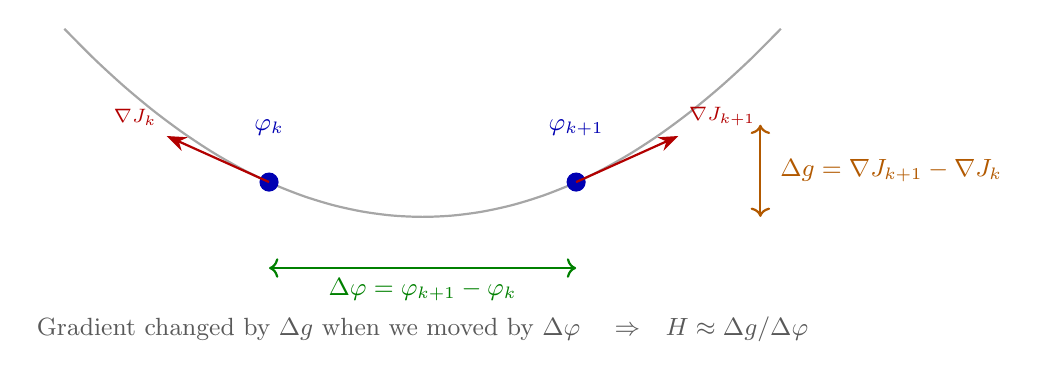
\begin{tikzpicture}[scale=1.3]
    % Curve (cost function along a 1D slice) — wider parabola
    \draw[thick, gray!70] plot[smooth, domain=-1:6] (\x, {0.15*(\x-2.5)*(\x-2.5) + 0.8});

    % Points on the curve
    \filldraw[blue!70!black] (1.0, 1.14) circle (2.5pt);
    \filldraw[blue!70!black] (4.0, 1.14) circle (2.5pt);

    % Point labels — well separated from arrows
    \node[blue!70!black, font=\small, above] at (1.0, 1.5) {$\varphi_k$};
    \node[blue!70!black, font=\small, above] at (4.0, 1.5) {$\varphi_{k+1}$};

    % Gradient arrows (tangent directions, pointing away from curve)
    \draw[thick, red!70!black, -{Stealth[length=2.5mm]}] (1.0, 1.14) -- (0.0, 1.59)
        node[above left, font=\scriptsize] {$\nabla J_k$};
    \draw[thick, red!70!black, -{Stealth[length=2.5mm]}] (4.0, 1.14) -- (5.0, 1.59)
        node[above right, font=\scriptsize] {$\nabla J_{k+1}$};

    % Delta phi (below curve)
    \draw[thick, green!50!black, <->] (1.0, 0.3) -- (4.0, 0.3)
        node[midway, below, font=\small] {$\Delta\varphi = \varphi_{k+1} - \varphi_k$};

    % Delta g (right side, well separated)
    \draw[thick, orange!70!black, <->] (5.8, 0.8) -- (5.8, 1.7);
    \node[orange!70!black, font=\small, right] at (5.9, 1.25) {$\Delta g = \nabla J_{k+1} - \nabla J_k$};

    % Secant condition label (below, with breathing room)
    \node[font=\small, align=center, text=gray!70!black] at (2.5, -0.3)
        {Gradient changed by $\Delta g$ when we moved by $\Delta\varphi$
         \quad$\Rightarrow$\quad $H \approx \Delta g / \Delta\varphi$};
\end{tikzpicture}
\caption{The quasi-Newton idea: observe how the gradient changes between steps. The ratio $\Delta g / \Delta\varphi$ gives information about the Hessian (curvature) without computing it directly.}
\label{fig:secant}
\end{figure}

\subsection{BFGS: The Best Quasi-Newton Update}

The BFGS update (Broyden--Fletcher--Goldfarb--Shanno, 1970) is a specific formula for updating the Hessian approximation $B_k$ at each step using the secant condition. It maintains two properties:
\begin{enumerate}
    \item $B_k$ is symmetric positive-definite (so the search direction is always downhill)
    \item $B_k$ satisfies the secant condition $B_k \Delta\varphi = \Delta g$ for the most recent step
\end{enumerate}

The update formula (you don't need to memorize this):
\begin{equation}
B_{k+1} = B_k - \frac{B_k\,\Delta\varphi\,\Delta\varphi^T\!B_k}{\Delta\varphi^T\!B_k\,\Delta\varphi} + \frac{\Delta g\,\Delta g^T}{\Delta g^T\Delta\varphi}
\end{equation}

In practice, we work with the \emph{inverse} Hessian approximation $B_k^{-1}$ directly (to avoid solving a linear system at each step).

\subsection{L-BFGS: The ``Limited Memory'' Version We Actually Use}

\textbf{Problem with BFGS:} Storing $B_k^{-1}$ requires $N_t^2$ memory. For $N_t = 8192$: 512~MB per matrix. Not terrible, but wasteful.

\textbf{L-BFGS solution:} Don't store $B_k^{-1}$ explicitly. Instead, store only the last $m$ pairs $\{(\Delta\varphi_i, \Delta g_i)\}_{i=k-m}^{k-1}$ (typically $m = 10$). When you need $B_k^{-1}\nabla J$ (the search direction), compute it on-the-fly using a clever two-loop recursion that only touches the stored pairs.

\textbf{Memory:} $O(m \cdot N_t)$ instead of $O(N_t^2)$. For $m = 10$, $N_t = 8192$: 640~KB vs.\ 512~MB.

\textbf{Cost per iteration:} One gradient evaluation (forward + adjoint $\approx 2$~s) plus $O(m \cdot N_t)$ linear algebra ($\approx 0.001$~s). The gradient dominates.

% ─── Memory comparison diagram ───────────────────────────────────────────
\begin{figure}[H]
\centering
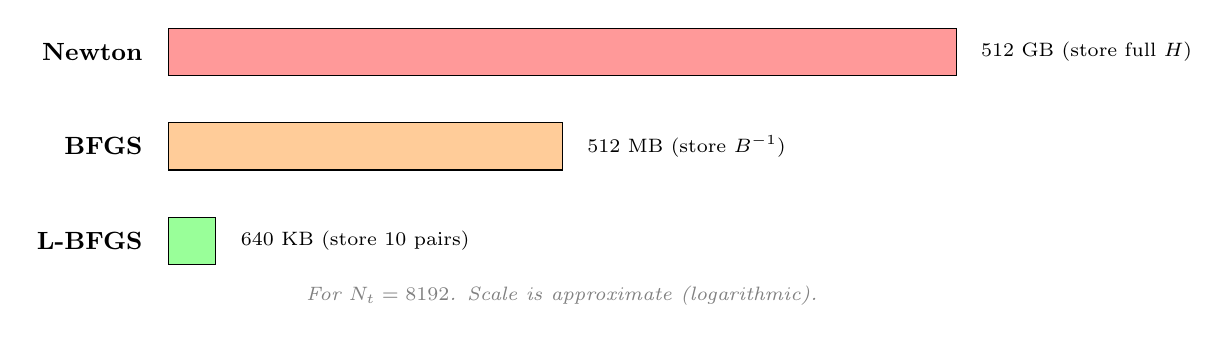
\begin{tikzpicture}[
    bar/.style={draw, minimum height=0.6cm, anchor=west, font=\small},
]
    % Labels
    \node[font=\small\bfseries, anchor=east] at (-0.2, 2.4) {Newton};
    \node[font=\small\bfseries, anchor=east] at (-0.2, 1.2) {BFGS};
    \node[font=\small\bfseries, anchor=east] at (-0.2, 0.0) {L-BFGS};

    % Bars (log scale visual)
    \node[bar, fill=red!40, minimum width=10cm] at (0, 2.4) {};
    \node[font=\scriptsize, anchor=west] at (10.2, 2.4) {512 GB (store full $H$)};

    \node[bar, fill=orange!40, minimum width=5cm] at (0, 1.2) {};
    \node[font=\scriptsize, anchor=west] at (5.2, 1.2) {512 MB (store $B^{-1}$)};

    \node[bar, fill=green!40, minimum width=0.6cm] at (0, 0.0) {};
    \node[font=\scriptsize, anchor=west] at (0.8, 0.0) {640 KB (store 10 pairs)};

    % Scale note
    \node[font=\scriptsize\itshape, text=gray] at (5, -0.7) {For $N_t = 8192$. Scale is approximate (logarithmic).};
\end{tikzpicture}
\caption{Memory comparison for $N_t = 8192$. Newton stores the full Hessian. BFGS stores an approximation. L-BFGS stores only 10 vector pairs --- nearly 1000$\times$ less memory than BFGS.}
\label{fig:memory}
\end{figure}

\begin{keyeq}
\textbf{The L-BFGS algorithm:}
\begin{enumerate}[leftmargin=*]
    \item Start with initial phase $\varphi_0$ (usually zeros)
    \item Compute gradient $\nabla J$ via forward + adjoint solve ($\sim$2~s)
    \item Compute search direction $d = -B_k^{-1}\nabla J$ using stored $(\Delta\varphi, \Delta g)$ pairs
    \item \textbf{Line search:} Find step size $\alpha$ satisfying the Wolfe conditions (sufficient decrease + curvature condition). This requires 1--3 additional forward evaluations.
    \item Update: $\varphi_{k+1} = \varphi_k + \alpha\,d$
    \item Store $(\Delta\varphi, \Delta g)$ pair; discard oldest if $> m$ pairs stored
    \item Repeat until $|\nabla J| < \text{tolerance}$ or iteration limit reached
\end{enumerate}
\end{keyeq}

\subsection{The Line Search: Picking the Step Size}

Even with a good direction $d$, we need to choose how far to step. Too far $\to$ overshoot. Too short $\to$ wasted iteration.

The \textbf{Wolfe conditions} define an acceptable step size $\alpha$:
\begin{align}
\text{Sufficient decrease:} \quad & J(\varphi + \alpha d) \leq J(\varphi) + c_1\,\alpha\,\nabla J \cdot d \label{eq:wolfe1}\\
\text{Curvature condition:} \quad & \nabla J(\varphi + \alpha d)\cdot d \geq c_2\,\nabla J \cdot d \label{eq:wolfe2}
\end{align}
with $0 < c_1 < c_2 < 1$ (typically $c_1 = 10^{-4}$, $c_2 = 0.9$).

Condition~\eqref{eq:wolfe1} says: ``the cost must decrease by at least a fraction $c_1$ of what we predicted.'' Condition~\eqref{eq:wolfe2} says: ``the gradient in the search direction must have flattened out enough'' (we're not stopping on a steep slope).

\begin{intuition}
The line search is like Goldilocks: the step must be long enough to make real progress (Wolfe 1) but not so long that we're climbing back up (Wolfe 2). In practice, the line search algorithm (Hager--Zhang in our code) uses cubic interpolation to find an acceptable $\alpha$ in 1--3 function evaluations.
\end{intuition}

% ─── Line search diagram ────────────────────────────────────────────────
\begin{figure}[H]
\centering
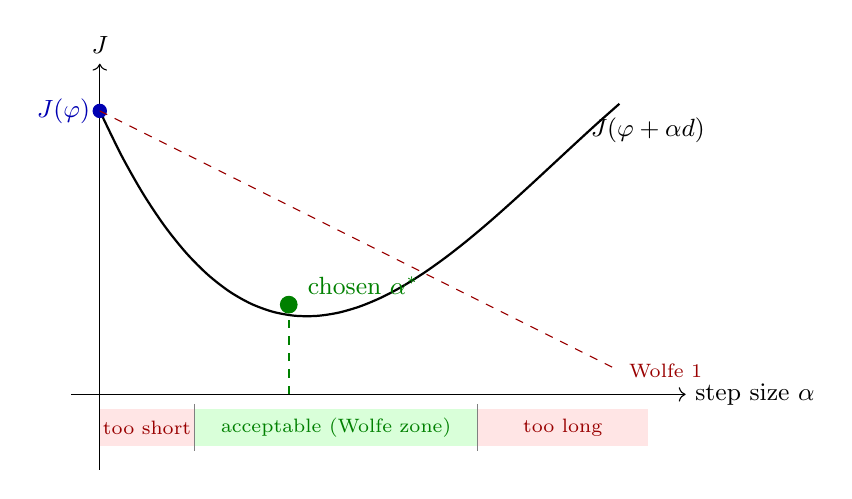
\begin{tikzpicture}[scale=1.2]
    % J(alpha) curve
    \draw[thick, black] plot[smooth, domain=0:5.5] (\x, {3 - 2.2*\x + 0.65*\x*\x - 0.045*\x*\x*\x});
    \node[font=\small] at (5.8, 2.8) {$J(\varphi + \alpha d)$};

    % Axes
    \draw[->] (-0.3, 0) -- (6.2, 0) node[right, font=\small] {step size $\alpha$};
    \draw[->] (0, -0.8) -- (0, 3.5) node[above, font=\small] {$J$};

    % Starting point
    \filldraw[blue!70!black] (0, 3) circle (2pt) node[left, font=\small] {$J(\varphi)$};

    % Sufficient decrease line (Wolfe 1)
    \draw[dashed, red!60!black] (0, 3) -- (5.5, 0.25) node[right, font=\scriptsize] {Wolfe 1};

    % Regions below x-axis with more room
    \fill[red!10] (0, -0.15) rectangle (1.0, -0.55);
    \node[font=\scriptsize, red!60!black] at (0.5, -0.35) {too short};

    \fill[green!15] (1.0, -0.15) rectangle (4.0, -0.55);
    \node[font=\scriptsize, green!50!black] at (2.5, -0.35) {acceptable (Wolfe zone)};

    \fill[red!10] (4.0, -0.15) rectangle (5.8, -0.55);
    \node[font=\scriptsize, red!60!black] at (4.9, -0.35) {too long};

    % Separator ticks
    \draw[gray] (1.0, -0.1) -- (1.0, -0.6);
    \draw[gray] (4.0, -0.1) -- (4.0, -0.6);

    % Chosen alpha
    \draw[thick, green!50!black, dashed] (2.0, 0) -- (2.0, 0.95);
    \filldraw[green!50!black] (2.0, 0.95) circle (2.5pt);
    \node[green!50!black, font=\small, above right] at (2.1, 0.95) {chosen $\alpha^*$};
\end{tikzpicture}
\caption{The line search finds a step size $\alpha^*$ in the ``Goldilocks zone'' (green): large enough to make real progress (below the Wolfe~1 line), but not so large that we overshoot past the minimum.}
\label{fig:linesearch}
\end{figure}

\subsection{Why L-BFGS Is Perfect for Our Problem}

\begin{center}
\begin{tabular}{lll}
\toprule
\textbf{Property} & \textbf{Our problem} & \textbf{Why L-BFGS wins} \\
\midrule
Dimension & $N_t = 8192$ & Too large for Newton ($N_t^2$ memory) \\
Gradient cost & 2~s (forward + adjoint) & Dominates; L-BFGS adds negligible overhead \\
Smoothness & PDE-based, $C^\infty$ & Quasi-Newton shines on smooth problems \\
Stochasticity & None (exact gradients) & No need for Adam/SGD robustness \\
Convergence & 20--60 iterations & Superlinear once Hessian approx is good \\
\bottomrule
\end{tabular}
\end{center}

In our runs, L-BFGS typically converges in 20--60 iterations $\times$ 2~s/iteration = \textbf{40~s to 2~min}. Gradient descent would take thousands of iterations for the same result.


% ═════════════════════════════════════════════════════════════════════════
\section{The Adjoint Method (The Key Insight)}

\subsection{Why Brute Force Fails}

To compute $\partial J/\partial\varphi_k$ via finite differences:
\begin{equation}
\pdv{J}{\varphi_k} \approx \frac{J(\varphi + \epsilon\,e_k) - J(\varphi - \epsilon\,e_k)}{2\epsilon}
\end{equation}
requires \textbf{two simulations per frequency}. With $N_t = 8192$: 16,384 simulations $\times$ 1~s each = \textbf{4.5 hours per gradient}. We need 30--60 gradients per optimization. That's weeks.

\subsection{The Adjoint Trick: Run the Movie Backwards}

\begin{intuition}
Instead of asking ``how does tweaking frequency $k$ affect the output?'' for each $k$, ask the reverse: ``given that we know what went wrong at the output, how did each input frequency contribute?'' One backward simulation answers \emph{all} 8192 questions simultaneously.
\end{intuition}

\textbf{Step 1 --- Forward:} Propagate $u_0 \to u_L$. Cost: 1 simulation (${\sim}1$~s).

\textbf{Step 2 --- Terminal condition:} Compute the ``error signal'' at the output:
\begin{equation}
\lambda_L(\omega) = \frac{u_L(\omega)\left[\mathbb{1}_\mathcal{B}(\omega) - J\right]}{E_{\text{total}}}
\label{eq:terminal}
\end{equation}
This encodes ``how much each output frequency contributed to the Raman cost.''

\textbf{Step 3 --- Adjoint:} Propagate $\lambda$ \emph{backward} from $z=L$ to $z=0$ through the same fiber (transposed/conjugated). Cost: 1 simulation (${\sim}1$~s).

\textbf{Step 4 --- Read off the gradient:}
\begin{keyeq}
\begin{equation}
\boxed{\pdv{J}{\varphi(\omega)} = 2\,\Real\!\left[\lambda_0^*(\omega)\cdot i\cdot u_0(\omega)\right]}
\label{eq:gradient}
\end{equation}
This is the complete gradient from \textbf{one forward + one backward simulation}: ${\sim}2$~s instead of 4.5 hours.
\end{keyeq}

\subsection{The Relay Race Analogy}

If a relay team lost, you could:
\begin{itemize}
    \item \textbf{Forward approach:} Replace each runner one at a time, re-run the race. Takes $N$ races.
    \item \textbf{Adjoint approach:} Start from the finish line, trace backward: ``lost 2~s in the last leg $\Leftarrow$ bad handoff in leg 3 $\Leftarrow$ runner 2 started late.'' One backward pass reveals every runner's contribution.
\end{itemize}

The adjoint equation implements this backward analysis for the GNLSE.

\subsection{The Adjoint Equation}

The adjoint field satisfies:
\begin{equation}
\dv{\lambda_\omega}{z} = -\left(\pdv{f}{u}\right)^\dagger \lambda - \left(\pdv{f}{u^*}\right)^T \lambda^*
\label{eq:adjoint}
\end{equation}
where $f$ is the GNLSE right-hand side. The $\dagger$ = conjugate transpose. Negative sign = backward integration.

For our GNLSE, this splits into four terms (from differentiating Kerr and Raman w.r.t.\ $u$ and $u^*$). You don't need to memorize them. They've been verified to \textbf{0.026\% accuracy} against finite differences.

\subsection{The Chain Rule}

The adjoint gives $\lambda_0$ = sensitivity to the input \emph{field}. But we control the \emph{phase}. Since $u_0 = u_{00}e^{i\varphi}$:
\begin{equation}
\delta u_0 = i\,u_0\,\delta\varphi \qquad\text{(derivative of $e^{ix}$ is $ie^{ix}$)}
\end{equation}
Substituting into the sensitivity formula gives Eq.~\eqref{eq:gradient}.


% ═════════════════════════════════════════════════════════════════════════
\section{The Log-Scale Trick}

\subsection{The Vanishing Gradient Problem}

When minimizing $J$ (a number between 0 and 1), the gradient shrinks as $J \to 0$:

\begin{warning}
At $J = 10^{-4}$, the gradient is $10^{-4}$ times as strong as at $J = 1$. The optimizer thinks it's converged --- but there's still 40~dB of room to improve. It's like walking downhill in fog: the ground flattens and you stop on a plateau.
\end{warning}

\subsection{The Fix: Optimize in Decibels}

Minimize $J_{\text{dB}} = 10\log_{10}(J)$ instead. The gradient becomes:
\begin{keyeq}
\begin{equation}
\pdv{J_{\text{dB}}}{\varphi} = \underbrace{\frac{10}{J\cdot\ln 10}}_{\text{amplification}} \cdot \pdv{J}{\varphi}
\label{eq:log_cost}
\end{equation}
As $J$ shrinks, the $1/J$ factor amplifies the gradient, exactly compensating the vanishing linear gradient.
\end{keyeq}

Going from $-40$~dB to $-50$~dB produces the same gradient magnitude as $0$~dB to $-10$~dB.

\textbf{Result:} 20--28~dB improvement on every configuration. Points stuck at $-35$~dB now reach $-60$~dB.

% ─── Log-cost comparison figure ────────────────────────────────────────
\begin{figure}[H]
\centering

\includegraphics[width=\textwidth]{fig3_linear_vs_log_cost.png}
\caption{Impact of the log-scale cost function on every SMF-28 sweep point. Orange bars: old linear cost (stuck at $-35$ to $-58$~dB). Blue bars: new log cost ($-37$ to $-78$~dB). Green numbers show improvement in dB. The last three points (L=5m) previously crashed with NaN.}
\label{fig:log_cost}
\end{figure}


% ═════════════════════════════════════════════════════════════════════════
\section{The Soliton Number}

Two length scales characterize pulse propagation:
\begin{align}
L_D &= \frac{T_0^2}{|\beta_2|} \quad\text{(dispersion length: how far until pulse doubles in width)} \\[4pt]
L_{NL} &= \frac{1}{\gamma P_{\text{peak}}} \quad\text{(nonlinear length: how far until nonlinear phase $= 1$~rad)}
\end{align}

The soliton number is their ratio:
\begin{keyeq}
\begin{equation}
N = \sqrt{\frac{L_D}{L_{NL}}} = \sqrt{\frac{\gamma P_{\text{peak}} T_0^2}{|\beta_2|}}
\end{equation}
\end{keyeq}

\begin{center}
\begin{tabular}{lll}
\toprule
$N$ & What happens & Suppression \\
\midrule
1.0--1.5 & Soliton-like propagation & Easy: $-60$ to $-78$~dB \\
1.5--2.5 & Pulse breathing, some compression & Moderate: $-50$ to $-70$~dB \\
2.5--4.0 & Soliton fission onset & Hard: $-45$ to $-65$~dB \\
4.0--7.0 & Full fission + Raman shifting & Harder: $-40$ to $-55$~dB \\
\bottomrule
\end{tabular}
\end{center}

% ─── Soliton regime TikZ ────────────────────────────────────────────────
\begin{figure}[H]
\centering
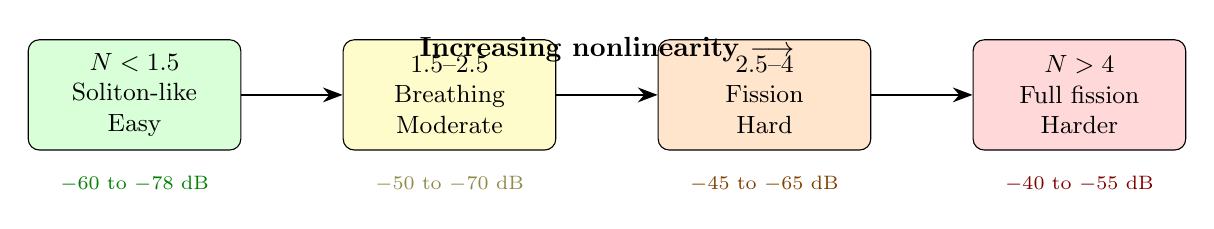
\begin{tikzpicture}[
    regime/.style={rectangle, draw, rounded corners, minimum width=2.7cm, minimum height=1.4cm, align=center, font=\small},
    arrow/.style={-{Stealth[length=2.5mm]}, thick}
]
\node[regime, fill=green!15] (low) at (0,0) {$N < 1.5$\\Soliton-like\\Easy};
\node[regime, fill=yellow!20] (mid) at (4,0) {$1.5$--$2.5$\\Breathing\\Moderate};
\node[regime, fill=orange!20] (high) at (8,0) {$2.5$--$4$\\Fission\\Hard};
\node[regime, fill=red!15] (ext) at (12,0) {$N > 4$\\Full fission\\Harder};

\draw[arrow] (low) -- (mid);
\draw[arrow] (mid) -- (high);
\draw[arrow] (high) -- (ext);

\node[above=0.3cm of $(low)!0.5!(ext)$, font=\bfseries] {Increasing nonlinearity $\longrightarrow$};
\node[below=0.2cm of low, font=\scriptsize, text=green!50!black] {$-60$ to $-78$~dB};
\node[below=0.2cm of mid, font=\scriptsize, text=yellow!50!black] {$-50$ to $-70$~dB};
\node[below=0.2cm of high, font=\scriptsize, text=orange!50!black] {$-45$ to $-65$~dB};
\node[below=0.2cm of ext, font=\scriptsize, text=red!50!black] {$-40$ to $-55$~dB};
\end{tikzpicture}
\caption{Soliton number regimes. Higher $N$ = stronger nonlinear dynamics = harder to suppress Raman. But the log-cost optimizer achieves $>40$~dB even at $N = 6.3$.}
\label{fig:soliton_regimes}
\end{figure}

% ─── N vs J scatter (real data) ─────────────────────────────────────────
\begin{figure}[H]
\centering

\includegraphics[width=0.85\textwidth]{fig2_nsol_vs_J.png}
\caption{Suppression vs.\ soliton number for all 24 sweep points. Color = fiber length (darker = shorter). Circles = SMF-28, squares = HNLF. The vertical spread at each $N$ comes from different fiber lengths --- fiber length, not $N$, is the dominant factor.}
\label{fig:nsol_scatter}
\end{figure}


% ═════════════════════════════════════════════════════════════════════════
\section{Wirtinger Derivatives Demystified}

\subsection{The Problem}

For $f(u, u^*)$ where $u = x + iy$: the standard complex derivative $df/du$ only exists if $f$ is analytic. But $|u|^2 = u\cdot u^*$ is \emph{not} analytic.

\subsection{Wirtinger's Solution}

Treat $u$ and $u^*$ as independent variables:
\begin{equation}
\pdv{f}{u} = \frac{1}{2}\!\left(\pdv{f}{x} - i\pdv{f}{y}\right) \qquad \pdv{f}{u^*} = \frac{1}{2}\!\left(\pdv{f}{x} + i\pdv{f}{y}\right)
\end{equation}

The key identity: $\partial|u|^2/\partial u^* = \partial(u\cdot u^*)/\partial u^* = u$. The $\partial/\partial u^*$ ``sees'' $u^*$ but treats $u$ as constant.

\subsection{The Factor of 2}

For real-valued $J$:
\begin{equation}
\delta J = \sum_k \pdv{J}{u_k}\delta u_k + \pdv{J}{u_k^*}\delta u_k^* = 2\,\Real\sum_k \pdv{J}{u_k^*}\delta u_k
\end{equation}

The 2 comes from combining the $u$ and $u^*$ terms. It's pure bookkeeping --- no physics.


% ═════════════════════════════════════════════════════════════════════════
\section{Why FFT Factors of $N_t$ Appear}

Julia's convention: \texttt{fft} = unnormalized ($\sum u_n e^{-2\pi ikn/N}$), \texttt{ifft} = normalized ($\frac{1}{N}\sum U_k e^{+2\pi ikn/N}$).

This means:
\begin{itemize}
    \item Adjoint of \texttt{fft} $= N_t \times$~\texttt{ifft}
    \item Adjoint of \texttt{ifft} $= (1/N_t) \times$~\texttt{fft}
\end{itemize}

That's where the $N_t$ factors in the adjoint code come from. Different FFT libraries use different conventions. The physics doesn't care, but the code must be self-consistent.


% ═════════════════════════════════════════════════════════════════════════
\section{Verification}

\subsection{Taylor Remainder Test}

Pick random $\delta\varphi$. Compute:
\begin{equation}
r(\epsilon) = |J(\varphi + \epsilon\,\delta\varphi) - J(\varphi) - \epsilon\,\nabla J\cdot\delta\varphi|
\end{equation}

If $\nabla J$ is correct, $r(\epsilon) \sim \epsilon^2$ (log-log slope = 2).

\textbf{Our result: slopes of 2.00 and 2.04.} The adjoint gradient matches the true gradient to machine precision.

\subsection{Finite Difference Check}

Compare adjoint gradient to central differences for each frequency. \textbf{Max relative error: 0.026\%.} Extremely accurate.


% ═════════════════════════════════════════════════════════════════════════
\section{What's Left in the Full Verification Document}

If you've followed this far, you understand the big picture. The remaining details are:
\begin{enumerate}
    \item \textbf{Term-by-term adjoint derivation:} Four terms from differentiating Kerr and Raman w.r.t.\ $u$ and $u^*$. Tedious but mechanical.
    \item \textbf{GDD penalty:} Penalizes curvature of $\varphi$. Standard finite-difference second derivative.
    \item \textbf{Boundary penalty:} Penalizes energy at window edges. Chain rule through IFFT.
\end{enumerate}
None contain surprising physics --- just careful bookkeeping of derivatives.


% ═════════════════════════════════════════════════════════════════════════
\section{The ML Connection}
\label{sec:ml}

\begin{mlbox}
The optimization is structurally identical to training a neural network. This isn't a loose analogy --- it's mathematically the same procedure.
\end{mlbox}

% ─── ML vs Physics pipeline diagram ─────────────────────────────────────
\begin{figure}[H]
\centering
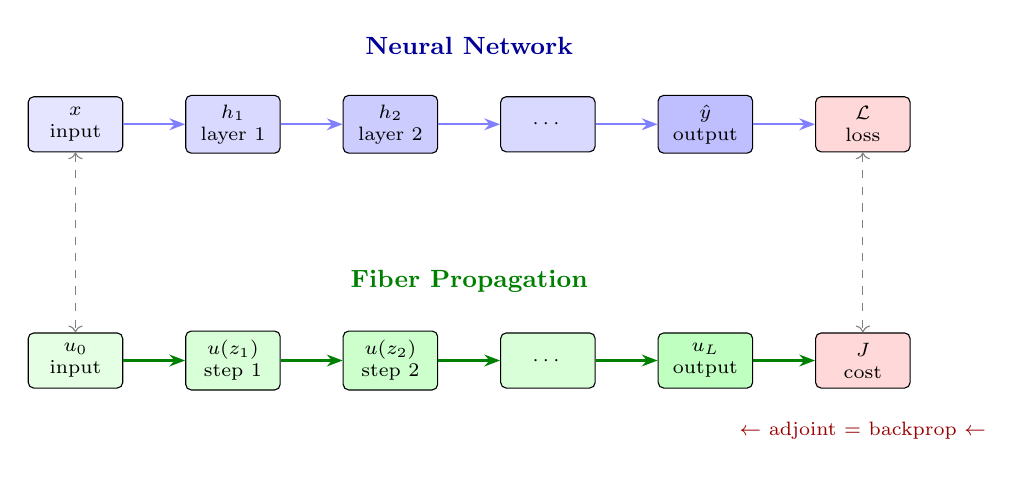
\begin{tikzpicture}[
    node distance=0.8cm and 1.2cm,
    layer/.style={rectangle, draw, rounded corners=2pt, minimum width=1.2cm, minimum height=0.7cm, align=center, font=\scriptsize},
    arrow/.style={-{Stealth[length=2mm]}, thick},
    label/.style={font=\scriptsize\itshape, text=gray}
]
% Neural network (top)
\node[font=\small\bfseries, blue!60!black] (nn_label) at (0, 2.5) {Neural Network};
\node[layer, fill=blue!10] (x) at (-5, 1.5) {$x$\\input};
\node[layer, fill=blue!15] (h1) at (-3, 1.5) {$h_1$\\layer 1};
\node[layer, fill=blue!20] (h2) at (-1, 1.5) {$h_2$\\layer 2};
\node[layer, fill=blue!15] (dots) at (1, 1.5) {$\cdots$};
\node[layer, fill=blue!25] (y) at (3, 1.5) {$\hat{y}$\\output};
\node[layer, fill=red!15] (loss) at (5, 1.5) {$\mathcal{L}$\\loss};

\draw[arrow, blue!50] (x) -- (h1);
\draw[arrow, blue!50] (h1) -- (h2);
\draw[arrow, blue!50] (h2) -- (dots);
\draw[arrow, blue!50] (dots) -- (y);
\draw[arrow, blue!50] (y) -- (loss);

% Fiber propagation (bottom)
\node[font=\small\bfseries, green!50!black] (fiber_label) at (0, -0.5) {Fiber Propagation};
\node[layer, fill=green!10] (u0) at (-5, -1.5) {$u_0$\\input};
\node[layer, fill=green!15] (uz1) at (-3, -1.5) {$u(z_1)$\\step 1};
\node[layer, fill=green!20] (uz2) at (-1, -1.5) {$u(z_2)$\\step 2};
\node[layer, fill=green!15] (dots2) at (1, -1.5) {$\cdots$};
\node[layer, fill=green!25] (uL) at (3, -1.5) {$u_L$\\output};
\node[layer, fill=red!15] (J) at (5, -1.5) {$J$\\cost};

\draw[arrow, green!50!black] (u0) -- (uz1);
\draw[arrow, green!50!black] (uz1) -- (uz2);
\draw[arrow, green!50!black] (uz2) -- (dots2);
\draw[arrow, green!50!black] (dots2) -- (uL);
\draw[arrow, green!50!black] (uL) -- (J);

% Equivalence arrows
\draw[<->, dashed, gray] (x.south) -- (u0.north) node[midway, left, label] {};
\draw[<->, dashed, gray] (loss.south) -- (J.north);

% Backward labels
\node[below=0.3cm of J, font=\scriptsize, red!60!black] {$\leftarrow$ adjoint $= $ backprop $\leftarrow$};
\end{tikzpicture}
\caption{Structural equivalence between neural network training and fiber optimization. Each ODE solver step in the fiber is analogous to one layer in a neural network. Backpropagation through layers $=$ adjoint propagation through the fiber.}
\label{fig:ml_analogy}
\end{figure}

\begin{center}
\begin{tabular}{lll}
\toprule
\textbf{ML Concept} & \textbf{Neural Network} & \textbf{Our Problem} \\
\midrule
Parameters & Weight matrices $W_k$ & Spectral phase $\varphi(\omega)$ \\
Input & Training data $x$ & Unshaped pulse $u_{00}$ \\
Forward pass & $x \to h_1 \to \cdots \to \hat{y}$ & $u_0 \to u(z_1) \to \cdots \to u_L$ \\
Loss function & Cross-entropy, MSE & $J = E_{\text{band}}/E_{\text{total}}$ \\
Backprop & Chain rule through layers & Adjoint solve through fiber \\
Optimizer & Adam, SGD, L-BFGS & L-BFGS \\
\bottomrule
\end{tabular}
\end{center}

\subsection{Forward Pass: Layers vs.\ Fiber Steps}

Neural net: $h_{k+1} = \sigma(W_k h_k + b_k)$.

Fiber: $u(z+\Delta z) = u(z) + \Delta z\cdot f(u(z), z)$.

Each $\Delta z$ step is one ``layer.'' The ``activation function'' is the GNLSE nonlinearity ($|u|^2 u$ + Raman convolution). There are ${\sim}1000$ ``layers'' (much deeper than most networks).

\subsection{Backprop = Adjoint}

In a neural net: $\delta_k = W_{k+1}^T\delta_{k+1}\cdot\sigma'(z_k)$. In our problem: $d\lambda/dz = -(\partial f/\partial u)^\dagger\lambda - \ldots$

Same structure: start with the loss gradient at the output, propagate backward through the same operations (transposed), get the gradient at the input.

\subsection{Why L-BFGS Instead of Adam?}

\begin{itemize}
    \item Our gradients are exact (no mini-batch noise).
    \item The problem is smooth (PDE, not piecewise-linear ReLU).
    \item L-BFGS builds a quadratic model of the loss --- much faster for smooth problems.
    \item Converges in 20--60 iterations vs.\ thousands for Adam.
\end{itemize}

\subsection{Log-Cost = Focal Loss}

Our $J_{\text{dB}} = 10\log_{10}(J)$ with gradient amplification $1/J$ is the same idea as \emph{focal loss} (Lin et al., 2017): downweight easy examples, amplify hard ones. As Raman gets suppressed (easy part done), the gradient amplifies to focus on remaining hard components.


% ═════════════════════════════════════════════════════════════════════════
\section{First Principles: Where the GNLSE Comes From}
\label{sec:first_principles}

\subsection{Maxwell's Equations}

Start from Maxwell in a dielectric:
\begin{equation}
\nabla\times\mathbf{E} = -\pdv{\mathbf{B}}{t} \qquad \nabla\times\mathbf{B} = \mu_0\pdv{\mathbf{D}}{t}
\end{equation}

The displacement field has a nonlinear part:
$\mathbf{D} = \epsilon_0\mathbf{E} + \mathbf{P}_L + \mathbf{P}_{NL}$
where $\mathbf{P}_L = \epsilon_0\chi^{(1)}\mathbf{E}$ is linear and $\mathbf{P}_{NL}$ contains $\chi^{(3)}$ (third-order susceptibility --- the lowest nonlinear order in glass, which is centrosymmetric so $\chi^{(2)} = 0$).

\subsection{Slowly-Varying Envelope Approximation}

Write the field as a carrier times a slowly-varying envelope:
\begin{equation}
E(z,t) = \tfrac{1}{2}\!\left[u(z,t)\,e^{i(\beta_0 z - \omega_0 t)} + \text{c.c.}\right]
\end{equation}

``Slowly varying'' means $|\partial u/\partial t| \ll \omega_0|u|$ and $|\partial u/\partial z| \ll \beta_0|u|$. Substituting into Maxwell and dropping $\partial^2 u/\partial z^2$:
\begin{equation}
\pdv{u}{z} + \beta_1\pdv{u}{t} = i\sum_{n\geq 2}\frac{\beta_n}{n!}\!\left(i\pdv{}{t}\right)^n\!u + i\gamma|u|^2 u
\end{equation}

Moving to the co-moving frame ($T = t - \beta_1 z$) eliminates $\beta_1$.

\subsection{Adding Raman}

The $\chi^{(3)}$ response has an instantaneous part (electrons) and a delayed part (nuclei, ${\sim}2000\times$ heavier, respond on ${\sim}30$~fs):
\begin{equation}
P_{NL}(t) = \epsilon_0\chi^{(3)}\!\left[(1-f_R)|u|^2 + f_R\!\int_0^\infty\!h_R(\tau)|u(t-\tau)|^2\,d\tau\right]u(t)
\end{equation}

This gives the full GNLSE (Eq.~\ref{eq:gnlse}). Every term traces back to Maxwell + silica material response.

\subsection{Where $\gamma$ and $h_R(t)$ Come From}

\begin{equation}
\gamma = \frac{n_2\omega_0}{c\cdot A_{\text{eff}}}
\end{equation}
where $n_2 \approx 2.6\times10^{-20}$~m$^2$/W (silica material property) and $A_{\text{eff}}$ is the mode area (fiber geometry). Smaller core $\Rightarrow$ more intense light $\Rightarrow$ stronger nonlinearity.

$h_R(t)$ is the impulse response of the Si--O--Si vibrational mode at ${\sim}13.2$~THz, modeled as a damped harmonic oscillator (Blow--Wood model). Quality factor $Q \approx 8.2$ (moderately underdamped).


% ═════════════════════════════════════════════════════════════════════════
\section{The Adjoint from First Principles}
\label{sec:adjoint_first_principles}

\subsection{Constrained Optimization via the Lagrangian}

Minimize $J[u_L]$ subject to $du/dz = f(u,z)$. Standard calculus of variations.

\textbf{Step 1:} Lagrangian with multiplier $\lambda(z)$:
\begin{equation}
\mathcal{L} = J[u_L] + \int_0^L\!\left\langle \lambda(z),\,\dv{u}{z} - f(u,z)\right\rangle dz
\end{equation}

\textbf{Step 2:} $\delta\mathcal{L}/\delta\lambda = 0$ $\Rightarrow$ forward equation. (No surprise.)

\textbf{Step 3:} Variation w.r.t.\ $u$:
\begin{equation}
\delta\mathcal{L} = \left\langle\pdv{J}{u_L},\delta u_L\right\rangle + \int_0^L\!\left\langle\lambda,\,\dv{(\delta u)}{z} - \pdv{f}{u}\delta u\right\rangle dz
\end{equation}

\textbf{Step 4:} Integration by parts on $\langle\lambda, d(\delta u)/dz\rangle$:
\begin{equation}
\int_0^L\!\left\langle\lambda,\dv{(\delta u)}{z}\right\rangle dz = \big[\langle\lambda,\delta u\rangle\big]_0^L - \int_0^L\!\left\langle\dv{\lambda}{z},\delta u\right\rangle dz
\end{equation}

\textbf{Step 5:} Choose $\lambda$ so the integral vanishes:
\begin{equation}
\dv{\lambda}{z} = -\left(\pdv{f}{u}\right)^\dagger\lambda \qquad\text{(the adjoint equation)}
\end{equation}

\textbf{Step 6:} Terminal condition $\lambda_L = -\partial J/\partial u_L^*$ kills the $z=L$ boundary.

\textbf{Step 7:} What's left: $\delta J = -\langle\lambda_0, \delta u_0\rangle$. Since $\delta u_0 = iu_0\delta\varphi$:
\begin{equation}
\delta J = 2\,\Real[\lambda_0^*\cdot i\cdot u_0]\cdot\delta\varphi \qquad\checkmark
\end{equation}

The adjoint equation arises naturally from integration by parts in the Lagrangian. QED.


% ═════════════════════════════════════════════════════════════════════════
% ═════════════════════════════════════════════════════════════════════════
\section{Results: What Does Suppression Look Like?}

These figures show actual results from our optimization sweep.

% ─── Evolution color map ─────────────────────────────────────────────────
\begin{figure}[H]
\centering

\includegraphics[width=\textwidth]{evolution_smf28_L2m_P02W.png}
\caption{\textbf{The money figure.} Pulse propagation through 2~m of SMF-28 at 0.20~W. \textbf{Left:} optimized pulse --- spectrum stays confined, Raman band (past the dashed line) is dark. \textbf{Right:} unshaped pulse --- clear soliton fission at $z \approx 0.5$~m and bright Raman sidelobe growing past 1600~nm. The optimizer found a phase that prevents the soliton compression that triggers Raman.}
\label{fig:evolution}
\end{figure}

% ─── Heatmaps ────────────────────────────────────────────────────────────
\begin{figure}[H]
\centering

\includegraphics[width=\textwidth]{fig1_heatmaps.png}
\caption{Full parameter sweep: Raman suppression across 24 configurations. Darker purple = better suppression. Each cell shows J in dB; asterisk = not formally converged. The dominant trend is top-to-bottom (fiber length), not left-to-right (power).}
\label{fig:heatmaps}
\end{figure}

% ─── Multistart ──────────────────────────────────────────────────────────
\begin{figure}[H]
\centering

\includegraphics[width=\textwidth]{fig4_multistart_comparison.png}
\caption{Robustness test: 10 optimizations from different random initial phases. \textbf{Left (old):} linear cost --- 0/10 converged, 28.6~dB spread. \textbf{Right (new):} log cost --- 10/10 converged, 10.9~dB spread. The apparent ``multiple local minima'' were an artifact of vanishing gradients, not true landscape complexity.}
\label{fig:multistart}
\end{figure}

% ─── Long fiber evolution ────────────────────────────────────────────────
\begin{figure}[H]
\centering

\includegraphics[width=\textwidth]{evolution_smf28_L5m_P01W.png}
\caption{Pushing the limits: 5~m of SMF-28 at 0.10~W. The unshaped pulse (right) shows massive spectral broadening by $z = 1$~m. The optimized pulse (left) keeps the spectrum contained through 5~m, though some leakage appears past $z = 3$~m --- this is where the input phase's influence starts to fade.}
\label{fig:evolution_5m}
\end{figure}


% ═════════════════════════════════════════════════════════════════════════
\section*{Quick Reference: The 5 Equations That Matter}

\begin{tcolorbox}[colback=gray!5,colframe=gray!50!black]
\begin{align}
&\textbf{1. Forward (GNLSE):} && \dv{u}{z} = iDu + i\gamma(1-f_R)|u|^2u + i\gamma f_R(h_R*|u|^2)u \\[8pt]
&\textbf{2. Cost function:} && J = \frac{E_{\text{Raman band}}}{E_{\text{total}}} \\[8pt]
&\textbf{3. Terminal condition:} && \lambda_L = \frac{u_L\cdot(\mathbb{1}_{\text{band}} - J)}{E_{\text{total}}} \\[8pt]
&\textbf{4. Gradient:} && \pdv{J}{\varphi(\omega)} = 2\,\Real[\lambda_0^*\cdot i\cdot u_0] \\[8pt]
&\textbf{5. Log-scale trick:} && \pdv{J_{\text{dB}}}{\varphi} = \frac{10}{J\ln 10}\cdot\pdv{J}{\varphi}
\end{align}
Everything else is implementation details.
\end{tcolorbox}

% ═════════════════════════════════════════════════════════════════════════
\section{What the April 2026 Parallel-Session Push Actually Showed}

Between 2026-04-16 and 2026-04-19 eight Claude-Code sessions ran in
parallel across a Mac laptop and two GCP VMs to pressure-test the
single-mode Raman-suppression result and begin the multimode
extension. The full synthesis is in
\texttt{results/SYNTHESIS-2026-04-19.md}; the physics audit filtering
those claims is in \texttt{results/PHYSICS\_AUDIT\_2026-04-19.md}.
This section reports only the findings that survived the audit.

\subsection{The suppression record, re-baselined}

On SMF-28 at $L = 0.5$~m and $P = 0.05$~W, the canonical
single-mode optimum is $J = -76.86$~dB (21 L-BFGS iterations, 25~s
wall-time, converged). The re-run matched the original Phase 10
baseline within 1~dB. Source: \texttt{results/raman/phase17/SUMMARY.md}
lines 41--48; data at \texttt{results/raman/phase17/baseline.jld2}.

\begin{intuition}
The number is stable across re-runs, solver seeds, and the determinism
fix (see §16.4). It is the most defensible single-mode number in
this project.
\end{intuition}

\subsection{The optimum is on a razor's edge}

How robust is that $-77$~dB? A 20-sample Gaussian perturbation of the
optimal phase at each of five standard deviations gives a \textbf{3~dB
degradation radius of $\sigma_{3\text{dB}} = 0.025$~rad}. That is
\emph{sharp}: an SLM (spatial light modulator, the device you would
actually use to put this phase on a pulse) with a typical calibration
envelope of $\geq 0.05$~rad rms would already lose most of the
suppression advantage.

\begin{warning}
``We found a $-77$~dB optimum'' and ``You can build a $-77$~dB shaper''
are \emph{not} the same statement. The optimum sits in a narrow well.
If you are going to use this in hardware, the tolerance number matters
as much as the optimum number.
\end{warning}

\subsection{The simple phase is a good \emph{initialiser}, not a universal minimum}

Two intuitions got tested against each other:
\begin{description}
  \item[``Simple phase is a universal attractor.''] Take the
    $-77$~dB phase from $L = 0.5$~m / $P = 0.05$~W and
    \emph{evaluate} (no re-optimisation) at 7 different
    (length, power) targets on SMF-28. Result: 0/7 stayed within
    3~dB of the warm-reopt value. The phase does not transfer as-is.
  \item[``Simple phase is a good warm start.''] Same seed phase,
    but now let L-BFGS re-optimise from it at each target. Result:
    11/11 nearby (fiber, $L$, $P$) configurations reached $-70$ to
    $-82$~dB in 6--40 iterations, \emph{including} HNLF at $-79.5$~dB
    (a fiber the baseline was never computed for).
\end{description}

The right framing is the second one: the simple phase lives in a
manifold of nearby basins, and moving to any of them takes a small
number of L-BFGS iterations. The simplicity is an
\emph{initialisation prior}, not a \emph{generalisation property}.

\subsection{Determinism}

Prior to this pass, two identical Julia processes with the same
\texttt{Random.seed!(42)} would produce different $\varphi_{\text{opt}}$
vectors (max $|\Delta\varphi| = 1.04$~rad, $\Delta J = 1.8$~dB).
Root cause: the code built FFT plans with \texttt{FFTW.MEASURE}, which
picks the fastest algorithm by \emph{timing} candidate plans under
live kernel noise; different runs, different plans, different
floating-point rounding, different L-BFGS trajectories.

Switching the planner to \texttt{FFTW.ESTIMATE} (deterministic
heuristic, no timing) gives \emph{bit-identical} $J$ across 3
independent processes. Cost: $+21.4\%$ wall time on the SMF-28
$L = 2$~m $P = 0.2$~W benchmark. Source:
\texttt{results/raman/phase15/benchmark.md} lines 20--27, 39.

\begin{intuition}
If two supposedly-identical runs disagree, look at the FFT planner
before you look at anything physical.
\end{intuition}

\subsection{What did \emph{not} survive}

Three claims that appeared in the 48-hour synthesis did not make it
through the audit:
\begin{itemize}
  \item A polynomial-fit comparison of $\varphi_{\text{opt}}$ between
    $L = 2$~m and $L = 100$~m was used to argue for ``nonlinear
    structural adaptation.'' The fit's $R^2$ was $0.015$ at 100~m
    and $0.037$ at 2~m --- in both cases the quadratic model
    explained less than 4\% of the phase variance, so the extracted
    $a_2$ coefficients are noise. A ratio of noise is noise.
    (See \texttt{PHYSICS\_AUDIT\_2026-04-19.md} §W1.)
  \item The 100~m L-BFGS ``optimum'' of $-54.77$~dB is a lower bound
    (25 iter, $\|\nabla J\| = 0.48$, \texttt{converged = false}),
    not a converged minimum. (Audit §S4.)
  \item A joint $\{\varphi, A, E\}$ L-BFGS that regressed from
    $-57$~dB to $-23$~dB is a preconditioning bug (mixed units), not
    physics. (Audit §M1.)
\end{itemize}

These are flagged here because the April push was widely circulated,
and future-you is likely to remember the numbers without remembering
which ones survived. If you see any of these three cited anywhere,
stop and check the audit.

% ═════════════════════════════════════════════════════════════════════════
\vspace{2em}
\hrule
\vspace{0.5em}
{\small\textit{Written as a companion to the formal verification document. Core math verified against the codebase on 2026-04-02; April 2026 integration findings (§16) reconciled against the audit on 2026-04-19.}}

\end{document}
